\documentclass[aspectratio=169]{beamer}\usepackage[]{graphicx}\usepackage[]{xcolor}
% maxwidth is the original width if it is less than linewidth
% otherwise use linewidth (to make sure the graphics do not exceed the margin)
\makeatletter
\def\maxwidth{ %
  \ifdim\Gin@nat@width>\linewidth
    \linewidth
  \else
    \Gin@nat@width
  \fi
}
\makeatother

\definecolor{fgcolor}{rgb}{0.345, 0.345, 0.345}
\newcommand{\hlnum}[1]{\textcolor[rgb]{0.686,0.059,0.569}{#1}}%
\newcommand{\hlsng}[1]{\textcolor[rgb]{0.192,0.494,0.8}{#1}}%
\newcommand{\hlcom}[1]{\textcolor[rgb]{0.678,0.584,0.686}{\textit{#1}}}%
\newcommand{\hlopt}[1]{\textcolor[rgb]{0,0,0}{#1}}%
\newcommand{\hldef}[1]{\textcolor[rgb]{0.345,0.345,0.345}{#1}}%
\newcommand{\hlkwa}[1]{\textcolor[rgb]{0.161,0.373,0.58}{\textbf{#1}}}%
\newcommand{\hlkwb}[1]{\textcolor[rgb]{0.69,0.353,0.396}{#1}}%
\newcommand{\hlkwc}[1]{\textcolor[rgb]{0.333,0.667,0.333}{#1}}%
\newcommand{\hlkwd}[1]{\textcolor[rgb]{0.737,0.353,0.396}{\textbf{#1}}}%
\let\hlipl\hlkwb

\usepackage{framed}
\makeatletter
\newenvironment{kframe}{%
 \def\at@end@of@kframe{}%
 \ifinner\ifhmode%
  \def\at@end@of@kframe{\end{minipage}}%
  \begin{minipage}{\columnwidth}%
 \fi\fi%
 \def\FrameCommand##1{\hskip\@totalleftmargin \hskip-\fboxsep
 \colorbox{shadecolor}{##1}\hskip-\fboxsep
     % There is no \\@totalrightmargin, so:
     \hskip-\linewidth \hskip-\@totalleftmargin \hskip\columnwidth}%
 \MakeFramed {\advance\hsize-\width
   \@totalleftmargin\z@ \linewidth\hsize
   \@setminipage}}%
 {\par\unskip\endMakeFramed%
 \at@end@of@kframe}
\makeatother

\definecolor{shadecolor}{rgb}{.97, .97, .97}
\definecolor{messagecolor}{rgb}{0, 0, 0}
\definecolor{warningcolor}{rgb}{1, 0, 1}
\definecolor{errorcolor}{rgb}{1, 0, 0}
\newenvironment{knitrout}{}{} % an empty environment to be redefined in TeX

\usepackage{alltt}
\usetheme{gotham}

	\usepackage{standalone}
	\usepackage{tikz}
	\usepackage{pgfplots}
	\usepackage{tabularray} % Typeset tabulars and arrays (contains equivalent of longtable, booktabs and dcolumn at least)
		\UseTblrLibrary{booktabs} % to load extra commands from booktabs
	\usepackage{changepage}
	\usepackage{minted}
		\definecolor{codeback}{rgb}{0.90,0.91,0.92}
		\definecolor{codebackdark}{rgb}{0.10,0.11,0.12}

	\newcommand{\famName}[1]{\textsc{#1}}
	\newcommand{\themename}{\textbf{\textsc{Gotham}}}
\IfFileExists{upquote.sty}{\usepackage{upquote}}{}
\begin{document}

\section{Informing Policy via Dynamic Models: Cholera in Haiti}

\begin{frame}{Introduction}
  \setbeamercovered{transparent}
  One of the most scientifically interesting types of SSMs are \emph{mechanistic models}.
  
  \begin{itemize}
    \item Used when we have some understanding of how a dynamic system evolves over time. 
    \item Useful in modern science, and have some advantages over machine learning models \citep{baker18,hogg24}:
    \begin{itemize}
      \item Accounting for known (but unobserved) features can improve model performance. 
      \item More intepretable. 
      \item Facilitates predictions of interventions and other counter-factuals. 
    \end{itemize}
  \end{itemize}
  \pause
  In this chapter, I demonstrate these capabilities by fitting mechanistic models to the 2010-2019 cholera outbreak in Haiti \citep{wheeler24}. 
\end{frame}

\begin{frame}{Cholera in Haiti}
 \begin{tabular}{cl}  
         \begin{tabular}{c}
           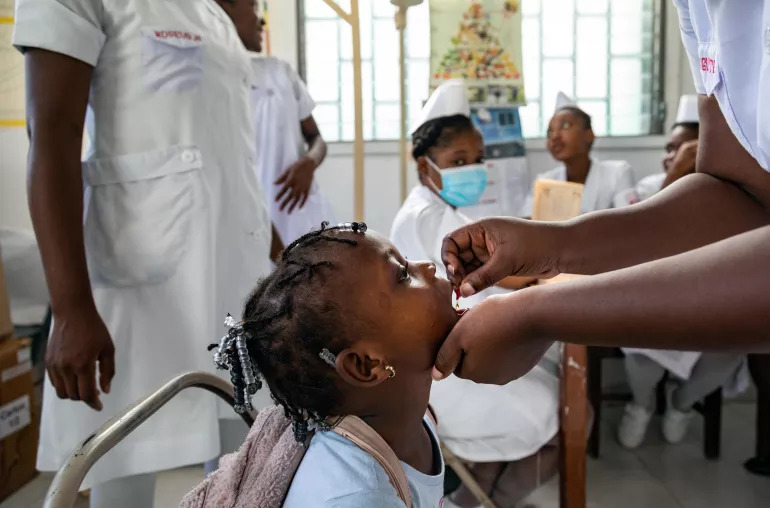
\includegraphics[height=4.3cm, width=5.5cm]{haiti/vaccination.jpeg}
           \end{tabular}
           & \begin{tabular}{l}
             \parbox{0.5\linewidth}{%  change the parbox width as appropiate
             \begin{itemize}
              \item Haiti experienced a cholera outbreak following the devastating 2010 earthquake. 
              \item From 2010-2019, more than \alert{800,000} recorded cases, making it one of the largest recorded outbreaks.
              \item Oral cholera vaccination (OCV) is available, but in limited supply.
              \item Image credit: \citet{unicef22}.
             \end{itemize}
    }
         \end{tabular}  \\
\end{tabular}
\end{frame}

\begin{frame}{Proposing interventions}
% At the time, there was interest in whether or not vaccinations would be a viable approach to eradicate cholera from Haiti.

A group of top researchers built three mechanistic models to estimate the potential impacts of various vaccination strategies \citep{lee20}.

\begin{itemize}
  \item The distinct teams each concluded predicted cholera resurgence from Feb 2019 - Feb 2024. 
  \item There were no confirmed cases from Feb 2019 - Sep 2022 \citep{trevisin22}. 
  \item Though there were some cases recently recorded, not near the predicted scale \citep{PAHO23}.
\end{itemize}

\alert{Questions:} What are strengths and weaknesses of mechanistic models? What are common mistakes researchers make? How can we improve outcomes in the future?

\end{frame}

\begin{frame}{Available Data}

\begin{knitrout}
\definecolor{shadecolor}{rgb}{0.969, 0.969, 0.969}\color{fgcolor}
\includegraphics[width=\maxwidth]{figure/plotHaitiData-1} 
\end{knitrout}
           
\end{frame}

\begin{frame}{Spatially explicit model: Model 3}

 \begin{tabular}{ll}  
         \begin{tabular}{l}
          %%%%% SEAIR diagram
  \resizebox{0.55\textwidth}{!}{
    \Large
    \setlength{\unitlength}{5pt}
    \begin{picture}(100,70)(1,15)

    % COMPARTMENTS
    \put(39, 50){\circle{6}}
    \put(37, 49){$\mathrm{W}_{u}$}

    \put(8, 55){\framebox(6, 6){$\mathrm{S_{u0}}$}}
    \put(8, 39){\framebox(6, 6){$\mathrm{S_{u\vaccCounter}}$}}
    \put(36, 62.5){\framebox(6, 6){$\mathrm{A_{u}}$}}
    \put(36, 31.5){\framebox(6, 6){$\mathrm{I_{u}}$}}
    \put(56, 55){\framebox(6, 6){$\mathrm{R^1_{u0}}$}}
    \put(71, 55){\framebox(6, 6){$\mathrm{R^2_{u0}}$}}
    \put(86, 55){\framebox(6, 6){$\mathrm{R^3_{u0}}$}}
    \put(56, 39){\framebox(6, 6){$\mathrm{R^1_{u\vaccCounter}}$}}
    \put(71, 39){\framebox(6, 6){$\mathrm{R^2_{u\vaccCounter}}$}}
    \put(86, 39){\framebox(6, 6){$\mathrm{R^3_{u\vaccCounter}}$}}

    % INDIVIDUAL MOVEMENT
    % S_u0 -> A_u
    \put(15, 58.5){\vector(3, 1.2){20}}

    % S_u0 -> I_u
    \put(15, 57.5){\vector(1, -1.1){20}}

    % S_uz -> I_u
    \put(15, 41.5){\vector(3, -1.2){20}}

    % S_uz -> A_u
    \put(15, 42.5){\vector(1, 1.1){20}}

    % I_u -> R_u0
    \put(43, 66){\vector(2, -1){12}}

    % A_u -> R_uz
    \multiput(43, 64)(1.25, -1.6){12}{\line(1, -1.3){0.7}}
    \put(57, 46){\vector(1, -1.3){0.2}}

    \put(43, 36){\vector(1.7, 2){15}}

    \multiput(60, 54)(0, -2){4}{\line(0, -1){1}}
    \put(60, 46){\vector(0, -1){0.5}}

    \multiput(74, 54)(0, -2){4}{\line(0, -1){1}}
    \put(74, 46){\vector(0, -1){0.5}}

    \multiput(89, 54)(0, -2){4}{\line(0, -1){1}}
    \put(89, 46){\vector(0, -1){0.5}}

    \put(63, 58){\vector(1, 0){7}}
    \put(78, 58){\vector(1, 0){7}}

    \put(63, 42){\vector(1, 0){7}}
    \put(78, 42){\vector(1, 0){7}}

    \multiput(39, 61.5)(0, -1){8}{\line(0, -1){0.3}}
    \put(39,54){\vector(0, -1){0.5}}

    \multiput(39, 38.5)(0, 1){8}{\line(0, 1){0.3}}
    \put(39,46){\vector(0, 1){0.5}}

    \cbezier(89,62)(80, 85)(20, 85)(12,62)
    \put(12.2,62.5){\vector(-1, -3.5){0.3}}

    \cbezier(89,38)(80, 15)(20, 15)(12,38)
    \put(12.2,37.5){\vector(-1, 3.5){0.3}}

    \multiput(11, 54)(0, -2){4}{\line(0, -1){1}}
    \put(11, 46){\vector(0, -1){0.5}}

    % DEMOGRAPHY
    % -> S
    \put(0, 58){\vector(1, 0){7}}
    \put(1, 59){$\mathrm{\mu_{\demography S_{u0}}}$}

    % S Death
    \put(10, 62){\vector(0, 1){7}}
    \put(8, 64){$\mathrm{\muDeath}$}
    \put(10, 38){\vector(0, -1){7}}
    \put(8, 34){$\mathrm{\muDeath}$}

    % A + I death
    \put(39, 69.5){\vector(0, 1){7}}
    \put(37, 71.5){$\mathrm{\muDeath}$}

    \put(39, 31.5){\vector(0, -1){7}}
    \put(30, 27.5){$\mathrm{\muDeath + \choleraDeath}$}

    % R Death
    \put(59, 62){\vector(0, 1){7}}
    \put(57, 64){$\mathrm{\muDeath}$}

    \put(74, 62){\vector(0, 1){7}}
    \put(72, 64){$\mathrm{\muDeath}$}

    \put(59, 38){\vector(0, -1){7}}
    \put(57, 34){$\mathrm{\muDeath}$}

    \put(74, 38){\vector(0, -1){7}}
    \put(72, 34){$\mathrm{\muDeath}$}

    \put(93, 42){\vector(1, 0){7}}
    \put(95.5, 43){$\mathrm{\muDeath}$}

    \put(93, 58){\vector(1, 0){7}}
    \put(95.5, 59){$\mathrm{\muDeath}$}

    % W death
    \multiput(43, 50)(1, 0){7}{\line(1, 0){0.2}}
    \put(50.2, 50){\vector(1, 0){0.5}}
    \put(44, 51){$\mathrm{\Wremoval}$}

    \end{picture}
  }  
         \end{tabular}
           & \begin{tabular}{l}
             \parbox{0.38\linewidth}{%  change the parbox width as appropiate
             \begin{itemize}
              \item Spatial Dependence between units.
              \item Stochastic transmission rates.
              \item Overdispersed Markov counting system.
              \item Rainfall driven transmission.
              \item Environmental reservoir of bacteria.
              \item Adjustments for Hurricane Mathew (Oct 2016).
             \end{itemize}
    }
         \end{tabular}  \\
\end{tabular}

\end{frame}

\begin{frame}{Model Fitting}
The iterated block particle filter (IBPF) was used to fit the model \citep{ionides24}.

\begin{table}[ht]
\centering
\begin{tabular}{|l|c|c|c|}
\hline
 & \textbf{Our Fit} & \textbf{Original Fit} & \textbf{Benchmark} \\
\hline
Log-likelihood & \cellcolor{green!20}-17332.9 & \cellcolor{red!20}-33832.6 & -17932.6 \\
\hline
AIC & \cellcolor{green!20}34733.9 & \cellcolor{red!20}67723.2 & 35945.0 \\
\hline
\end{tabular}
\caption{Comparison of our fitted model to original parameters used to inform vaccination policy.}
\label{tab:fit_comparison}
\end{table}

\end{frame}

\begin{frame}{Key findings}

\begin{itemize}
  \item Confirmed importance of rainfall and reduced transmission over time.
  \item Importance of proper model diagnostics.
  \begin{itemize}
    \item Comparing to benchmarks.
    \item Checking results against features of the system. 
  \end{itemize}
  \item Reproducibility and Extendability. 
  \item Confirmed previous findings: stochastic models are better descriptions of the system, and over-dispersed models are best.
\end{itemize}

\end{frame}

\end{document}
%EoF
